%------------------------------------------%
% Saturday Morning Statistics
% Date: 12/25/2021
%------------------------------------------%
\documentclass[xcolor={dvipsnames}]{beamer}
\hypersetup{pdfpagemode=FullScreen}
\mode<presentation>{
  \usetheme{Boadilla}
  \usecolortheme{orchid}
  \usefonttheme{default}
  \setbeamertemplate{navigation symbols}{}
  \setbeamertemplate{caption}[numbered]
} 
\usepackage[english]{babel}
\usepackage[utf8x]{inputenc}
\setbeamersize{text margin left=0.5in,text margin right=0.5in}

\usepackage[dvipsnames]{xcolor}
\definecolor{DarkGreen}{RGB}{2, 48, 32}
\definecolor{CalyxGreen}{RGB}{34, 153, 84}
\definecolor{DarkOrange}{RGB}{199, 0, 57}
\definecolor{LightOrange}{RGB}{255, 87, 51}
\definecolor{LightGreen}{RGB}{218, 247, 166}
\definecolor{LightYellow}{RGB}{255, 195, 0}

\setbeamercolor*{palette primary}{bg=LightGreen, fg = DarkGreen}
\setbeamercolor*{palette secondary}{bg=LightGreen, fg=DarkGreen}
\setbeamercolor*{palette tertiary}{bg=LightGreen, fg = DarkGreen}
%\setbeamercolor*{palette quaternary}{bg=myNewColorD, fg = green}

%------------------------------------------%
% Packages
%------------------------------------------%
\usepackage{amsmath}
\renewcommand*\footnoterule{} %No sperating line on footnote
\usepackage{mathtools} %ANNOTATING EQUATIONS
\usepackage{hhline} %DOUBLBARS
\usepackage[super]{nth}
\usepackage{graphicx, caption, subcaption}

%------------------------------------------%
% Commands
%------------------------------------------%
\newcommand\T{\rule{0pt}{2.5ex}} %TOPSTRUT
\newcommand\B{\rule[-1.25ex]{0pt}{0pt}} %BOTTOMSTRUT
\newenvironment<>{varblock}[2][.9\textwidth] %RESIZED BLOCKS
  {\setlength{\textwidth}{#1}
  \begin{actionenv}#3
    \def\insertblocktitle{#2}\par
    \usebeamertemplate{block begin}}
  {\par\usebeamertemplate{block end}
  \end{actionenv}}
\defbeamertemplate{enumerate item}{largeball} %LARGE BALLS
{\begin{pgfpicture}{-1ex}{-0.65ex}{1.5ex}{1.5ex}
\usebeamercolor[fg]{item projected}
{\pgftransformscale{2.5}\pgftext{\Large\pgfuseshading{bigsphere}}}
{\pgftransformshift{\pgfpoint{0pt}{0.5pt}}
\pgftext{\usebeamerfont*{item projected}\small\insertenumlabel}}
\end{pgfpicture}}
\usepackage{tikz} % FANCY ARROWS
\usepackage{xparse}
\NewDocumentCommand\UpArrow{O{2.0ex} O{black}}{%
   \mathrel{\tikz[baseline] \draw [->, line width=0.5pt, #2] (0,0) -- ++(0,#1);}} % FANCY UPARROW
\NewDocumentCommand\DownArrow{O{2.0ex} O{black}}{%
   \mathrel{\tikz[baseline] \draw [<-, line width=0.5pt, #2] (0,0) -- ++(0,#1);}} % FANCY DOWNARROW
%\vskip 1cm
\makeatletter
\newcommand{\LeftEqNo}{\let\veqno\@@leqno}%LEFT EQUATION #'s
\makeatother

%------------------------------------------%
% Title
%------------------------------------------%
\title[\textbf{Saturday Morning Statistics}]{}
\author{Cannabis Data Science}
\institute[]{\Large Saturday Morning Statistics}
\date{December \nth{25}, 2021 \newline Christmas Day}
\begin{document}
\begin{frame}{}
  
\includegraphics[scale=0.075]{images/logos/cannlytics_logo_with_text_light.png}
  \titlepage
\end{frame}

%------------------------------------------%
% Introduction
%------------------------------------------%

\section{Introduction}

%------------------------------------------%
% Box-Jenkins Forecasting Methodology
%------------------------------------------%

\begin{frame}{}

{\large \textbf{The Box-Jenkings Forecasting Methodology}}\vspace{0.5\baselineskip}\\

\vspace{1\baselineskip}

\begin{enumerate}

\item Identification

\vspace{.5\baselineskip}

\item Estimation

\vspace{.5\baselineskip}

\item Diagnostic Checking

\vspace{.5\baselineskip}

\item Forecasting

\end{enumerate}


\end{frame}

%------------------------------------------%
% Step 1: Identification
%------------------------------------------%

\begin{frame}{}

{\large \textbf{Step 1: Identification}}\vspace{0.5\baselineskip}\\

\vspace{1\baselineskip}

Identify the order of an ARIMA (p, d, q) model.

\vspace{1\baselineskip}

\begin{itemize}

\item Analyze autocorrelation functions (ACFs) and partial autocorrelation functions (PACFs).

\vspace{.5\baselineskip}

\item Utilize statistical software to scan (p, d, q) models to select based on a selection criterion.

\end{itemize}

\end{frame}

%------------------------------------------%
% Step 2: Estimation
%------------------------------------------%

\begin{frame}{}

{\large \textbf{Step 2: Estimation}}\vspace{0.5\baselineskip}\\

\vspace{1\baselineskip}

Simply estimate the ARIMA(p, d, a) model that you identified.

\end{frame}

%------------------------------------------%
% Step 3: Diagnostic Checking
%------------------------------------------%

\begin{frame}{}

{\large \textbf{Step 3: Diagnostic Checking}}\vspace{0.5\baselineskip}\\

\vspace{1\baselineskip}

Examine if the residuals from the model are \textbf{white noise}. Why?

\vspace{1\baselineskip}

\begin{itemize}

\item The idea is that if the residuals are white noise, then there is no additional information that the model could explain.

\vspace{.5\baselineskip}

\item If the error are not white noise, then it is implied that there is still a presence of autocorrelation that can be explained by a different order ARIMA(p, d, q) model.
\end{itemize}

\end{frame}

%------------------------------------------%
% Step 4: Forecasting
%------------------------------------------%

\begin{frame}{}

{\large \textbf{Step 4: Forecasting}}\vspace{0.5\baselineskip}\\

\vspace{1\baselineskip}

Finally, forecast your target variable with your chosen model.

\vspace{1\baselineskip}

\begin{itemize}

\item Useful for short-term forecasting (up to a few months ahead).

\vspace{.5\baselineskip}

\item Difficult for long-term forecasting, because the model does not capture the state of the economy.

\end{itemize}

\end{frame}

%------------------------------------------%
% Forecasting
%------------------------------------------%

\begin{frame}{}

{\large \textbf{The 10 Commandments of Forecasting}}
\vspace{1\baselineskip}

{\scriptsize Silvia, J, Iqbal, A, et. al (2014), ‘Economic and Business Forecasting’.}

\vspace{1\baselineskip}

\begin{enumerate}
\item Know what you are forecasting.
\item Understand the purpose of forecasting.
\item Acknowledge the cost of the forecast error.
\item Rationalize the forecast horizon.
\item Understand the choice of variables.
\item Rationalize the forecasting model used.
\item Know how to present the results.
\item Know how to decipher the forecast results.
\item Use recursive methods.
\item Understand that forecasting models evolve over time.
\end{enumerate}
\end{frame}

%------------------------------------------%
% RMSE
%------------------------------------------%

\begin{frame}{}

{\large \textbf{Measuring Forecast Error}}\vspace{0.5\baselineskip}\\

\vspace{1\baselineskip}

The out-of-sample root mean square error (RMSE) can quantify forecast error.

\vspace{1\baselineskip}

$$
RMSE = \sqrt{\frac{1}{T}\Sigma(Y_{t+1} - \hat{Y}_{t+1})^2}
$$
\end{frame}

%------------------------------------------%
% Extensions
%------------------------------------------%

\begin{frame}{}

{\large \textbf{Model Extensions}}\vspace{0.5\baselineskip}\\

\vspace{1\baselineskip}

\begin{itemize}

\item Add exogenous fixed effects, such as month effects.

\vspace{0.5\baselineskip}

\item Add seasonality.

\vspace{0.5\baselineskip}

\item Use Bayesian methods.

\end{itemize}

\end{frame}

%------------------------------------------%
% Panel Data
%------------------------------------------%
%\section{Panel Data}
%
%\begin{frame}{}
%
%{\large \textbf{Panel Data}}\vspace{0.5\baselineskip}\\
%
%A panel has the form
%
%\begin{figure}
%    \begin{subfigure}[t]{.5\textwidth}
%      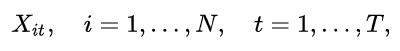
\includegraphics[width=\textwidth]{images/panel.png}
%    \end{subfigure}
%\end{figure}
%
%where $i$ is the individual dimension and $t$ is the time dimension.\vspace{0.5\baselineskip}\\
%
%A general panel data regression model is written as
%
%\begin{figure}
%    \begin{subfigure}[t]{.3\textwidth}
%      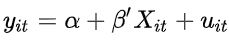
\includegraphics[width=\textwidth]{images/regression.png}
%    \end{subfigure}
%\end{figure}
%
%where
%
%\begin{figure}
%    \begin{subfigure}[t]{.25\textwidth}
%      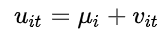
\includegraphics[width=\textwidth]{images/errors.png}
%    \end{subfigure}
%\end{figure}
%
%Estimation with a \textbf{fixed effects} or \textbf{random effects} model depends on assumptions about $\mu_i$, the individual-specific, time-invariant effects.
%
%\end{frame}

%------------------------------------------%
% Takeaway
%------------------------------------------%

\begin{frame}{}

\begin{center}
\begin{minipage}{3.85in}


\includegraphics[width=.25in]{images/prayer.png} {\Large \textbf{Thank you for coming.}}\vspace{0.5\baselineskip}\\

Take some time, discuss any conclusions drawn, and try to make some forecasts of your own!


\end{minipage}
\end{center}


\end{frame}

%------------------------------------------%
% References
%------------------------------------------%

\begin{frame}{}

{\large \textbf{References}}\vspace{0.5\baselineskip}\\

{\scriptsize Silvia, J, Iqbal, A, et. al (2014), ‘Economic and Business Forecasting’.}

\end{frame}

%------------------------------------------%
% Finale
%------------------------------------------%
\end{document}
